\newpage
\section{Data Collection}
\label{sec:datacollection}


This section explains how the data needed for the identification of \LEGO parameters was collected. It also includes a brief description of the code used.

\subsection{Code}
\label{sec:code}

Here a brief description of the code used to collect the data including the various modules used is given.
\subsubsection{ \LEGO Client}
\label{sec:client}



The \LEGO client module is programmed using \NXT and is written in C. It uses bluetooth to communicate with a server running on a PC to receive commands for controlling the motor and sending back the results. The data packets exchanged is of type \BTPKT and it contains the following fields:
\newline
\begin{itemize}
	\item  \textbf{size} : This stores the size of the packet. Its of type \UITT
    \item \textbf{packets} : This is an array of size \textbf{MAX\_REQ} which holds individual requests send to/from the \LEGO client. Its of type \BTREQ . The \BTREQ type contains the following fields:
    \begin{itemize}
    \item \textbf{operation} : The operation that's to be performed by \LEGO . This operation can either be to set the \textbf{motor power} or to fetch the current \textbf{Tacho count} of the motor.
    \item \textbf{port} : The \LEGO port onto which the request should be fowarded to.
    \item \textbf{data} : An array of size \textbf{MAX\_NUM\_DATA} which contains data sent to/from the \LEGO . \newline For setting the motor power, only the first index is used and it contains the power value to be set. However for fetching the tacho count, the first index contains the tacho count itself while the second index contains the timestamp when data was fetched.
    \end{itemize}
    
\end{itemize}

\subsubsection{Server}
\label{sec:server}

The server runs on the \textbf{PC} and it uses an \textbf{AF\_UNIX} socket to receive requests from a \textbf{Controller}, also running on the PC which issues the commands to be fowarded \LEGO . Its sole purpose is to act as a gateway between the \LEGO and the \textbf{Controller}.

\subsubsection{Controller}
\label{sec:controller}
The controller application runs on the PC and it uses an \textbf{AF\_UNIX} socket to communicate to the server. It allows for the possibility to automatically set a given range of power values and store the tacho count data for each given power in a text file.
\newline
Its main  functions include:
\begin{itemize}
	\item Decoding of command line arguments. These arguments include:
    	\begin{itemize}
        	\item Port number: This is th port number on which the motor is connected to the \LEGO . its preceded with \textbf{-p}.
            \item Power range: This is the range of the power values we wish to set to the motor. It contains three values delimited by \textbf{':'}. These values are the minimum power, maximum power and the step size(ie. Difference between each successive power value).Its preceded by \textbf{-m} .e.g. -m MIN\_POWER:MAX\_POWER:STEP\_SIZE 
            \item Number of samples : This value specifies the number of samples to be fetched for each power value set to the motor. Its preceded by \textbf{-m}.
        \end{itemize}
     \item Settting the motor power. It prepares packets to be sent to the \LEGO for altering the power values of the motor.
     \item Fetching the tacho count. The controller prepares and sends packets for feching the motor tacho counts and then logs the data in a text file. The format of the text file is as follows:
     \newline
     \hfill \textlangle tacho count\textrangle  \textlangle timestamp \textrangle \textlangle power value \textrangle
\end{itemize}
Between each subsequent power change, the motor power is set back to 0 and setting the next power value is delayed by 5 seconds to allow for the motor to rest and increase the accuracy of the data.

\subsection{Collecting the Data}
\label{sec:data}

Five sets of three thausand samples(3000) each was collected for ten different power values. In order to minimize the noise in the data, the five sets of data for each power value was averaged to produce the values to be used for analysis and identification of the motor parameters. The power values used is from ten to a hundred respectively.
\newline
The averaging was done using a scicos script and the results saved in text files: one for each power value in the same format as the original files.

\subsubsection{Data Filtering}
\label{sec:dataFiltering}
The data is filtered using an exponential low pass filter.

\begin{equation}
y(n) = \alpha x(n) + (1 - \alpha)x(n-1)
\end{equation}
\newline
An $\alpha$ value of 0.575 is used to perform the filtering.
\newline
The filtered data is them used in for parameter identification.
\begin{figure}
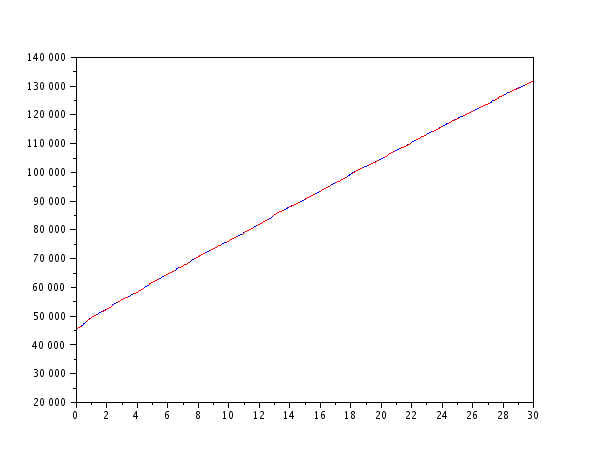
\includegraphics[scale=0.5]{images/10_dat_orig+filtered.png}
\caption{A graph showing filtered tacho count data with power value=10}
\end{figure}

\begin{figure}
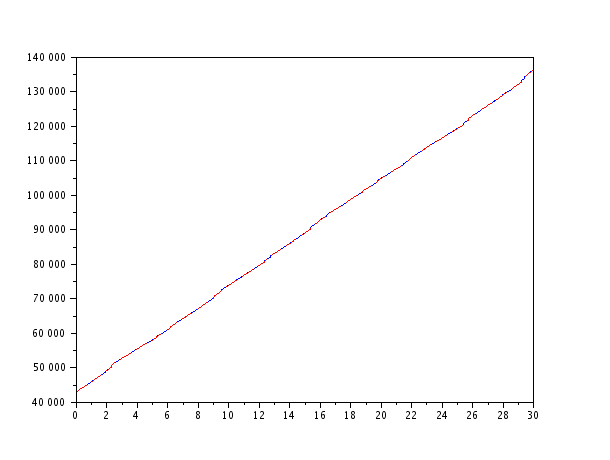
\includegraphics[scale=0.5]{images/100_dat_orig+filtered.png}
\caption{A graph showing filtered tacho count data with power value=100}
\end{figure}





